\section{Ejercicio 1}
El ejercicio consiste en programar una tarea que simule n llamadas bloqueantes (con n pasado por parámetro) donde la duración de cada llamada bloqueante está determinada por los parámetros bmin y bmax.

Para generar las duraciones al azar dentro del rango [bmin, bmax], se utilizó la funcion rand de la libreria stdlib y se realizó lo siguiente:\\

int cant = bmax - bmin + 1; \\
int cant_ciclos_bloqueada;\\
cant_ciclos_bloqueada = bmin + (rand() \% cant);\\

De esta forma se garantiza que $cant\_ciclos\_bloqueada$ esté entre el rango pedido.
Para realizar la simulación de las llamadas bloqueantes se ultilizó la función uso_IO provista por la cátedra.

Para probar la tarea se crearon los siguientes lotes:

\begin{itemize}
\item TaskConsola 5 10 20 
\item TaskConsola 15 2 20 
\end{itemize}

En la primera tarea se eligieron esos parámetros para comprobar que la cantidad de tiempo bloqueado respetara los límites requeridos, dado que la primera simulación no permitía apreciar gráficamente a simple vista la variabilidad dentro del rango, se creo la segunda tarea, con un rango más amplio para que el diagrama de Gantt manifieste dicha variabilidad en los tiempos de bloqueo random de la tarea.

\begin{figure}[h]
  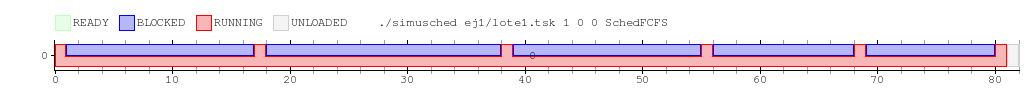
\includegraphics[width=\textwidth]{../ej1/lote1.png}
  \caption{Lote con 1 core, sin context switch. Sched.: FCFS}
\end{figure}

\begin{figure}[h]
  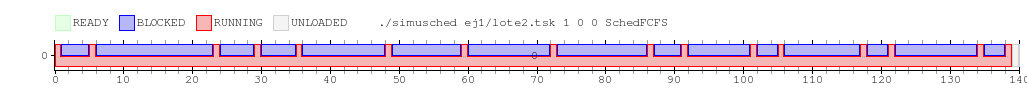
\includegraphics[width=\textwidth]{../ej1/lote2.png}
  \caption{Lote con 1 core, sin context switch. Sched.: FCFS}
\end{figure}